\chapter{Motivation}\label{ch:motivation}
This chapter examines existing literature concerning source recovery from Electroencephalography (EEG) measurements. 
At first a motivation for the source recovery problem is given, considering the application within the hearing aid industry. 
Further, the state of the art methods are presented followed by a description of the contribution proposed in this thesis.

\section{EEG Measurements}\label{sec:EEG}
EEG is a technique used within the medical field. 
It is an imaging technique measuring electric signals on the scalp, caused by brain activity. 
The human brain consist of an enormous amounts of cells, called neurons. 
These neurons are mutually connected in neural nets and when a neuron is activated, for instance by a physical stimuli, local current flows are produced \cite{fundamentalEEG}. This is also considered as a neural interaction across different parts of the human brain.   
\\ 
EEG measurements are provided by a number of metal electrodes, referred to as sensors, carefully placed on a human scalp. 
Each sensor reads the present electrical signals over time.
\\
It takes a large amount of active neurons to generate an electrical signal that is recordable on the scalp as the current have to penetrate the skull, skin and several other thin layers.
Hence it is clear that the EEG measurements from a single sensor do not correspond to the activity of one specific neuron in the brain, but rather a collection of many activities within the range of the one sensor.
Nor is the range of a single sensor separated from the other sensors. Thus the same activity can easily be measured by two or more sensors.
Furthermore, interfering signals can occur in the measurements resulting from physical movement of e.g. eyes and jawbone \cite{fundamentalEEG}. 
Lastly, the transmission of the electric field through the biological tissue to the sensor has an unknown mixing effect on the signal. This process is called volume conduction \cite[p. 68]{EEGsignalprocessing} \cite{Van2019}.
\\
This clarifies the mixture of electrical signals with noise that form the EEG measurements. 
The concept is sought illustrated on figure \ref{fig:volumeconduction}. 
\\
It will be clear later that it is of interest to separate and localize the sources of the neural activities measured on the scalp.  
\\ 
The waves resulting from EEG measurements are classified within four groups according to the dominant frequency. 
The delta wave ($0.5-4$ Hz) is observed from infants and sleeping adults, the theta wave ($4-8$ Hz) is observed from children and sleeping adults, the alpha wave ($8-13$ Hz) is the most extensively studied brain rhythm, which is induced by an adult laying down with closed eyes. 
Lastly, the beta wave ($13-30$ Hz) is considered the normal brain wave for adults, associated with active thinking, active attention or solving concrete problems \cite[p. 11]{EEGsignalprocessing}. 
An example of EEG measurements within the four categories is illustrated by figure \ref{fig:EEG_example}.        
\begin{figure}[H]
    \begin{minipage}[t]{.45\textwidth}
        \centering
        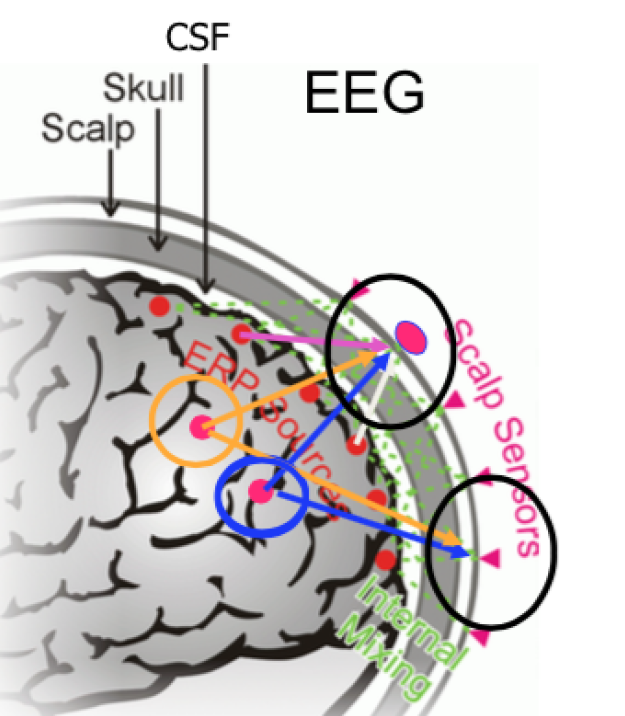
\includegraphics[width=\textwidth]{figurs/scalp.png}
        \caption{Illustration of volume conduction, source: \cite{phd2015}(we will make our own figure here instead)}\label{fig:volumeconduction}
    \end{minipage} 
    \hfill
    \begin{minipage}[t]{.45\textwidth}
        \centering
        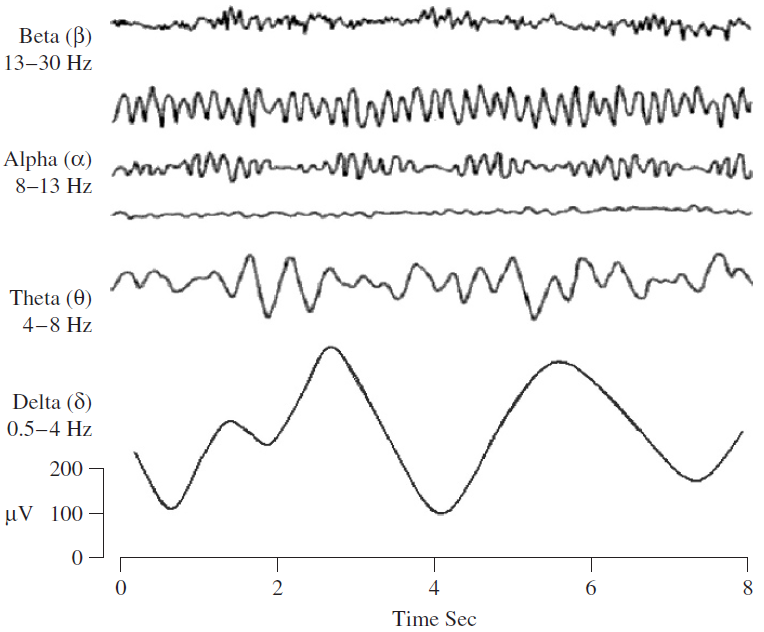
\includegraphics[width=\textwidth]{figurs/EEG_example.png}
        \caption{Example of time dependent EEG measurements within the four defined categories, source: \cite{EEGsignalprocessing}}\label{fig:EEG_example}
    \end{minipage}
\end{figure}
\noindent
EEG is widely used in the medical field, especially within research of the cognitive processes in the brain. 
Diagnosis and management of neurological disorders such as epilepsy is one example of application.
\\
EEG capitalizes on the procedure being non-invasive and fast.
Neural activity can be measured within fractions of a second after a stimuli has been provided \cite[p. 3]{fundamentalEEG}. 
When a person is exposed to a certain stimulus, e.g. visual or audible, the measured activity is said to result from evoked potential.
Over the past two decades, functional integration has become an area of interest \cite{Friston2011}. 
Within neurobiology functional integration refers to the study of the correlation among activities in different regions of the brain. 
In other words, how do different parts of the brain work together to process information and conduct a response \cite{Friston2002}.     
For this purpose separation and localization of the single sources which contribute to the EEG measurement is of interest. 
An article from 2016 \cite{Van2019} points out the importance of performing analysis regarding functional integration at source level rather than at EEG level. 
It is argued through experiments that analysis at EEG level does not allow interpretations about the interaction between sources.  
\\ 
The hearing aid industry is one example where this research is highly prioritized. 
At Eriksholm research center, which is a part of the hearing aid manufacturer Oticon, cognitive hearing science is a research area within fast development \cite{Weberik}. 
One main purpose at Eriksholm is to make it possible for a hearing aid to identify the user-inttended sound source and thereby exclude noise from elsewhere \cite{Emina2019} \cite{Bech2018}. 
This is where EEG and occasionally so called in-ear EEG is interesting, especially in conjunction with the technology of beamforming. With beamforming it is possible for a hearing aid to receive only signals from a specific direction. 
It is essentially the well known but unsolved cocktail problem which is sought improved by use of EEG. 
%However, the focus of this research is the correlation between EEG measurements and the sound source rather than localization of the activated source from the EEG \cite{Emina2019}. 
%Hence a source localization approach could potentially be of interest regarding hearing aids in order to improve the results.
%(Furthermore, a real-time application to provide feedback from EEG measurements would be essential.)\todo{?}. 


\subsection{Modelling}
Consider the issue of localizing activated sources from EEG measurements. A known approach is to model the observed data by the following linear system 
\begin{align*}
\mathbf{Y} = \mathbf{AX}.
\end{align*}
$\mathbf{Y} \in \mathbb{R}^{M \times L}$ is the EEG measurements of $L$ samples over time each consisting of $M$ measurements, one for each sensor. $\mathbf{A} \in \mathbb{R}^{M \times N}$ is an unknown mixing matrix and $\mathbf{X} \in \mathbb{R}^{N \times N_d}$ is makes the actual activation of sources within the brain. 
The $i$-th column of $\mathbf{A}$ represent the relative projection weights from the $i$-th source to every sensor \cite{phd2015}. 
This is in general referred to as a multiple measurement vector model. 
The aim in this case is to identify both $\mathbf{A}$ and $\mathbf{X}$ given the measurements $\mathbf{Y}$. 
For this specific set up is referred to as the EEG inverse problem.  
\\ \\
To solve the EEG inverse problem the concept of sparse signal recovery makes a solid foundation, including compressive sensing and dictionary learning. 
Independent Component Analysis (ICA) is a commonly applied method to solve the inverse problem \cite{Scott1996}, \cite{Scott1997}. Here statistical independence between source activity is the essential assumption. 
\\
Application of ICA have shown great results regarding source separation of high-density EEG. 
%Furthermore, an enhanced signal-to-noise ratio of the unmixed independent source time series processes allow essential study of the behaviour and relationships between multiple EEG source processes \cite{Arnaud2012}. 
\\
However, a significant flaw to this method is that the EEG measurements are only separated into a number of sources that are equal or less than the number of sensors \cite{Balkan2015}.
This means that the EEG inverse problem can not be over-complete. 
That is an assumption which undermines the reliability and usability of ICA, as the number of simultaneous active sources easily exceed the number of sensors \cite{phd2015}. 
This is especially a drawback when low-density EEG are considered, that is EEG equipment with less than 32 sensors. 
Improved capabilities of low-density EEG devices are desirable due to its relative low cost, mobility and ease to use. 
\\ \\
This makes a foundation to look at the existing work considering the over-complete inverse EEG problem. 

\section{Related Work and Our Contribution} 
As mentioned above ICA has been a solid method for source localization in the case where a separation into a number of sources equal to the number of sensors was adequate. 
To overcome this issue an extension of ICA was suggested, referred to as the ICA mixture model \cite{Balkan2015}.
Instead of identifying one mixing matrix $\mathbf{A} \in \mathbb{R}^{M \times N}$ this approach learns $N_{\text{model}}$\todo{(number of sources? or datapoints)} different mixing matrices $\mathbf{A}_i \in \mathbb{R}^{M\times M}$. 
The method was further adapted into the Adaptive Mixture ICA (AMICA) which showed successful results regarding identification of more sources than available sensors \cite{Palmer2008}. 
However an assumption of no more than $M$ simultaneously active sources has to be made which is still an essential limitation, especially when considering low-density EEG. 
\\
Other types of over-complete ICA algorithms have been proposed to overcome the problem of learning over-complete systems. 
One is the Restricted ICA (RICA), an efficient method used for unsupervised learning in neural networks \cite{Le2011}. 
Here the hard orthonormal constraint in ICA is replaced with a soft reconstruction cost.
\\
In 2015 O. Balkan et. al., \cite{Balkan2015}, suggested a new approach also targeting the identification of more sources than sensors regarding EEG. 
The suggested method, referred to as Cov-DL, is a covariance based dictionary learning algorithm. 
The point is to transfer the forward problem\todo{(?)} into the covariance domain, which has higher dimensionality than the original EEG sensor domain. 
This can be done when assuming the scalp mixing is linear and using the assumed natural non-correlation of sources within a certain time-window. 
The Cov-DL algorithm stands out from the other straight forward dictionary learning methods as it does not relay on the sparsity of active sources, this is an essential advantage when low-density EEG is considered. 
\\
Cov-DL was tested on found to outperform both AMICA and RICA \cite{Balkan2015}, thus it is considered the state of the art within the area of source identification. 
\\ \\
It is essential to note that the Cov-DL algorithm do only learn the mixing matrix $\mathbf{A}$, the projection of sources to the scalp sensors, and not the explicit source activity time series $\mathbf{X}$.
\\
For this purpose a multiple measurement sparse bayesian learning (M-SBL) algorithm was proposed in \cite{Balkan2014} also by O. Balkan et. al., also targeting the case of more active sources than sensors \cite{Balkan2014}. 
Here the mixing matrix which is known should fulfil the exact support recovery conditions. 
Though, the method was proven to outperform the recently used algorithm M-CoSaMP\todo{Find ud af hvad forkortelsen står for} even when the defined recovery conditions was not fulfilled.  
\\ \\
The two state of the art methods for source identification makes the foundation of this thesis. 
This thesis propose an algorithm with the purpose of solving the EEG inverse problem using the presented methods on EEG measurement. 
To extent the existing results the algorithm is expanded into a real-time application, in order to provide feedback based on the source activity.
\\
The intention of the feedback is to adjust the direction of the beam within the hearing aid depending on the source activity.      
For this, the application is tested within a simulation environment where the receiving direction of the test person can be adjusted in real-time. 
The quality of the final results is measured by the capability of improving the listener experience and the time used to proved useful feedback. 
\\ \\
As such our contribution \textit{(hopefully)} consists of tests of existing methods on new real-time measurement and furthermore include a feedback to control the microphone beam on a hearing aid. \todo{note: Evt. kunne vi lave en figur der lidt ala mindmap sætte et system overblik op og så highlighte de "bokse" vi vælger at arbejde med.}
